\chapter*{Add Noise Plugin}
\setcounter{chapter}{1}
\emph{Add some noise}
\section{Introduction}
The purpose of the \emph{AddNoise} plugin is to introduce random noise to \emph{Tellurium} data. 

Generation of actual noise is using the fact that a Rayleigh-distributed random variable $R$, with
the probability distribution $F(R) = 0$ if $R < 0$ and $F(R) = 1 - exp(-R^2/2*\sigma^2)$ if $R >= 0, $
is related to a pair of Gaussian variables $C$ and $D$ through the transformation $C = R * cos(\theta)$ and
$D = R * sin(\theta)$, where $\theta$ is a uniformly distributed variable
in the interval $(0, 2*\pi())$ \footnote{From Contemporary Communication Systems
USING MATLAB(R), by John G. Proakis and Masoud Salehi, published by
PWS Publishing Company, 1998, pp 49-50.} 

Currently only Gaussian noise is implemented. 

\section{Plugin Parameters}
Table \ref{table:AddNoisePluginParameters} lists available plugin property names, along with their data type and purpose.


\begin{table}[ht]
\centering % used for centering table
\begin{tabular}{l l p{7.5cm}} % centered columns (4 columns)

Parameter Name & Data Type & Purpose \\ [0.5ex] % inserts table 
%heading
\hline % inserts single horizontal line
InputData         		& 	TelluriumData & Data on which noise will be applied to. \\
Sigma,($\sigma$)      	& 	double & Size of applied noise. Noise is generated for each single data value, with a probability corresponding to a Gaussian distribution, centered around the value, and with a variance equal to $\sigma^2$ .\\
NoiseType      	& 	int    & Type of noise applied on data. Only Gaussian noise is currently supported. \\
Progress     	& 	double  & The progress property communicates the progress (in percent) of Noise application. \\

\hline %inserts single line
\end{tabular}
\caption{Add noise Plugin Parameters} 
\label{table:AddNoisePluginParameters} 
\end{table}

\section{Plugin Events}
The AddNoiseplugin are using all of a plugins available plugin events, i.e. the \emph{PluginStarted}, \emph{PluginProgress} and the \emph{PluginFinished} events.

The available data variables for each event are internally treated as \emph{pass trough} variables, so any data, for any of the events, assigned prior to 
the plugins execute function (in the assingOn() family of functions), can be retrieved \emph{unmodified} in the corresponding event function.
\begin{table}[ht]
\centering % used for centering table
\begin{tabular}{l l p{7.5cm}} % centered columns (4 columns)

Event & Arguments & Purpose \\ [0.5ex] % inserts table 
%heading
\hline % inserts single horizontal line
\hline % inserts single horizontal line
PluginStarted  	& 	void*, void*  & Signal to application that the plugin has started applying noise on data. Both parameters are \emph{pass trough} parameters and are unused internally by the plugin.\\[0.5ex]
PluginProgress	& 	void*, void*  & Communicating progress of noise generation. Both parameters are \emph{pass trough} parameters and are unused internally by the plugin. \\[0.5ex]
PluginFinished	& 	void*, void*  & Signals to application that execution of the plugin has finished. Both parameters are \emph{pass trough} parameters and are unused internally by the plugin.\\

\hline %inserts single line
\end{tabular}
\caption{AddNoise Plugin Events} 
\label{table:AddNoisePluginEvents} 
\end{table}

\section{The \texttt{execute(bool inThread)} function}
The \verb|execute()| function will apply noise to all rows and columns of the assigned data, with one exception. Data not affected are data in the first column, and if, and only if, its column header equals "time" (case insensitive). 

The \verb|execute(bool inThread)|, do support a boolean argument indicating if the execution of the plugin work will be done in a thread, or not. Threading is fully implemented in the AddNoise plugin.

The inThread argument defaults to \textbf{false}.

\section{Python examples}

\subsection{Add noise to data acquired from RoadRunner}
The python script below shows how to acquire simulation data from RoadRunner and pass it to the noise plugin. The format of the data, that is obtained from the \verb|simulate()| function (line 8), is not directly compatible with the Noise plugins InputData property. This incompatibility is handled by an intermediate data structure in Python, that is called DataSeries (line 14). 

The Plugins properties, InputData and Sigma, is assigned on line 17 and 20 respectively. 

Line 23 denote the execution of the noise plugin, and after that has finished, data can be visualized by using the \verb|plot| function (line 26). The output is shown below the script. 

\begin{singlespace}
\lstinputlisting[label=plugin_addNoise_header,caption={Add noise example.},language=Python]{Examples/telNoisePluginEx1.py}
\end{singlespace}

\begin{figure}[H]
\centering
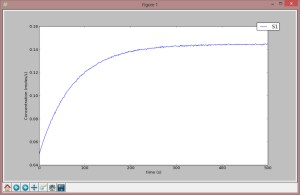
\includegraphics[angle=90,width=120mm]{AddNoise.jpg}
\caption{Output for the AddNoise python example script discussed above}
\label{fig:addNoiseFig1}
\end{figure}

\subsection{Visualization of the noise distribution used in the AddNoise plugin}
The Python script below demonstrate how to obtain and visualize the actual distribution (Gaussian) of noise that is applied on data.

\begin{singlespace}
\lstinputlisting[label=plugin_addNoise_header,caption={Noise distribution example.},language=Python]{Examples/telNoisePluginEx2.py}
\end{singlespace}

\begin{figure}[H]
\centering
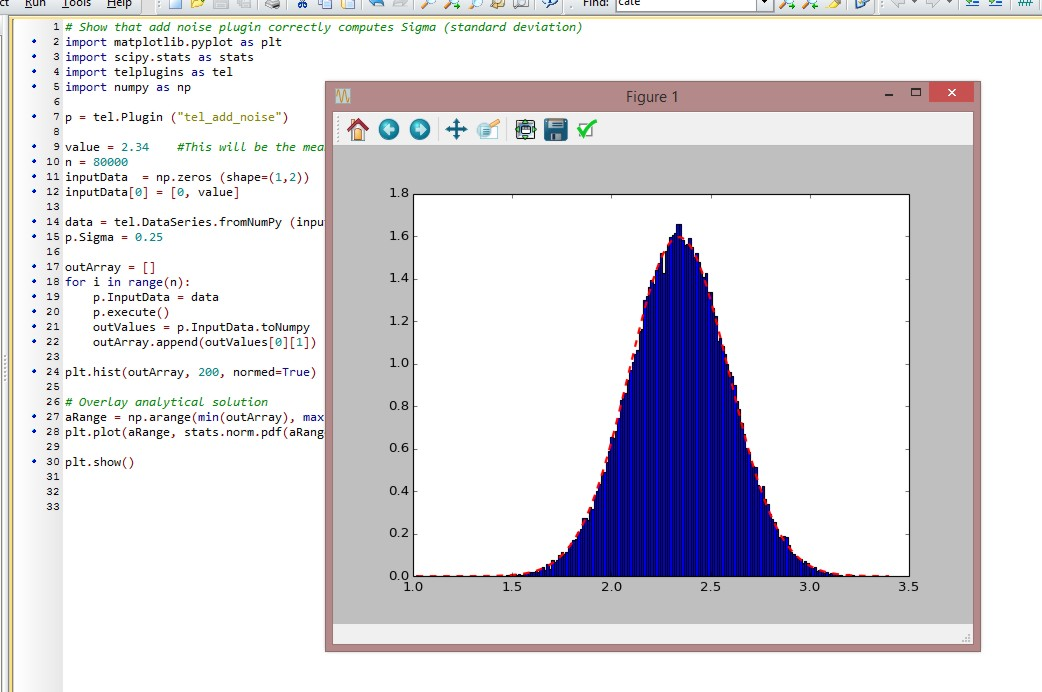
\includegraphics[angle=90,width=120mm]{AddNoise2.jpg}
\caption{Output for the AddNoise python example script discussed above}
\label{fig:addNoiseFig2}
\end{figure}

 






